\begin{frame}
% \frametitle{Объект исследования}
\textbf{Компьютерная томография} --- 

неразрушающий метод исследования внутренней структуры образцов.
\\ 
Применения:
\begin{itemize}
  \item Контроль качества изготавливаемых изделий
  \item Медицинская диагностика
  \item Использование результатов КТ для дальнейшего моделирования динамических процессов
  \item Биологические и геологические исследования
\end{itemize}

\end{frame}

\begin{frame}
% \frametitle{Объект исследования}
\centering
Томографическое измерение:
\begin{tabular}{p{0.45\textwidth} p{0.55\textwidth}}
  \begin{figure}[H]
    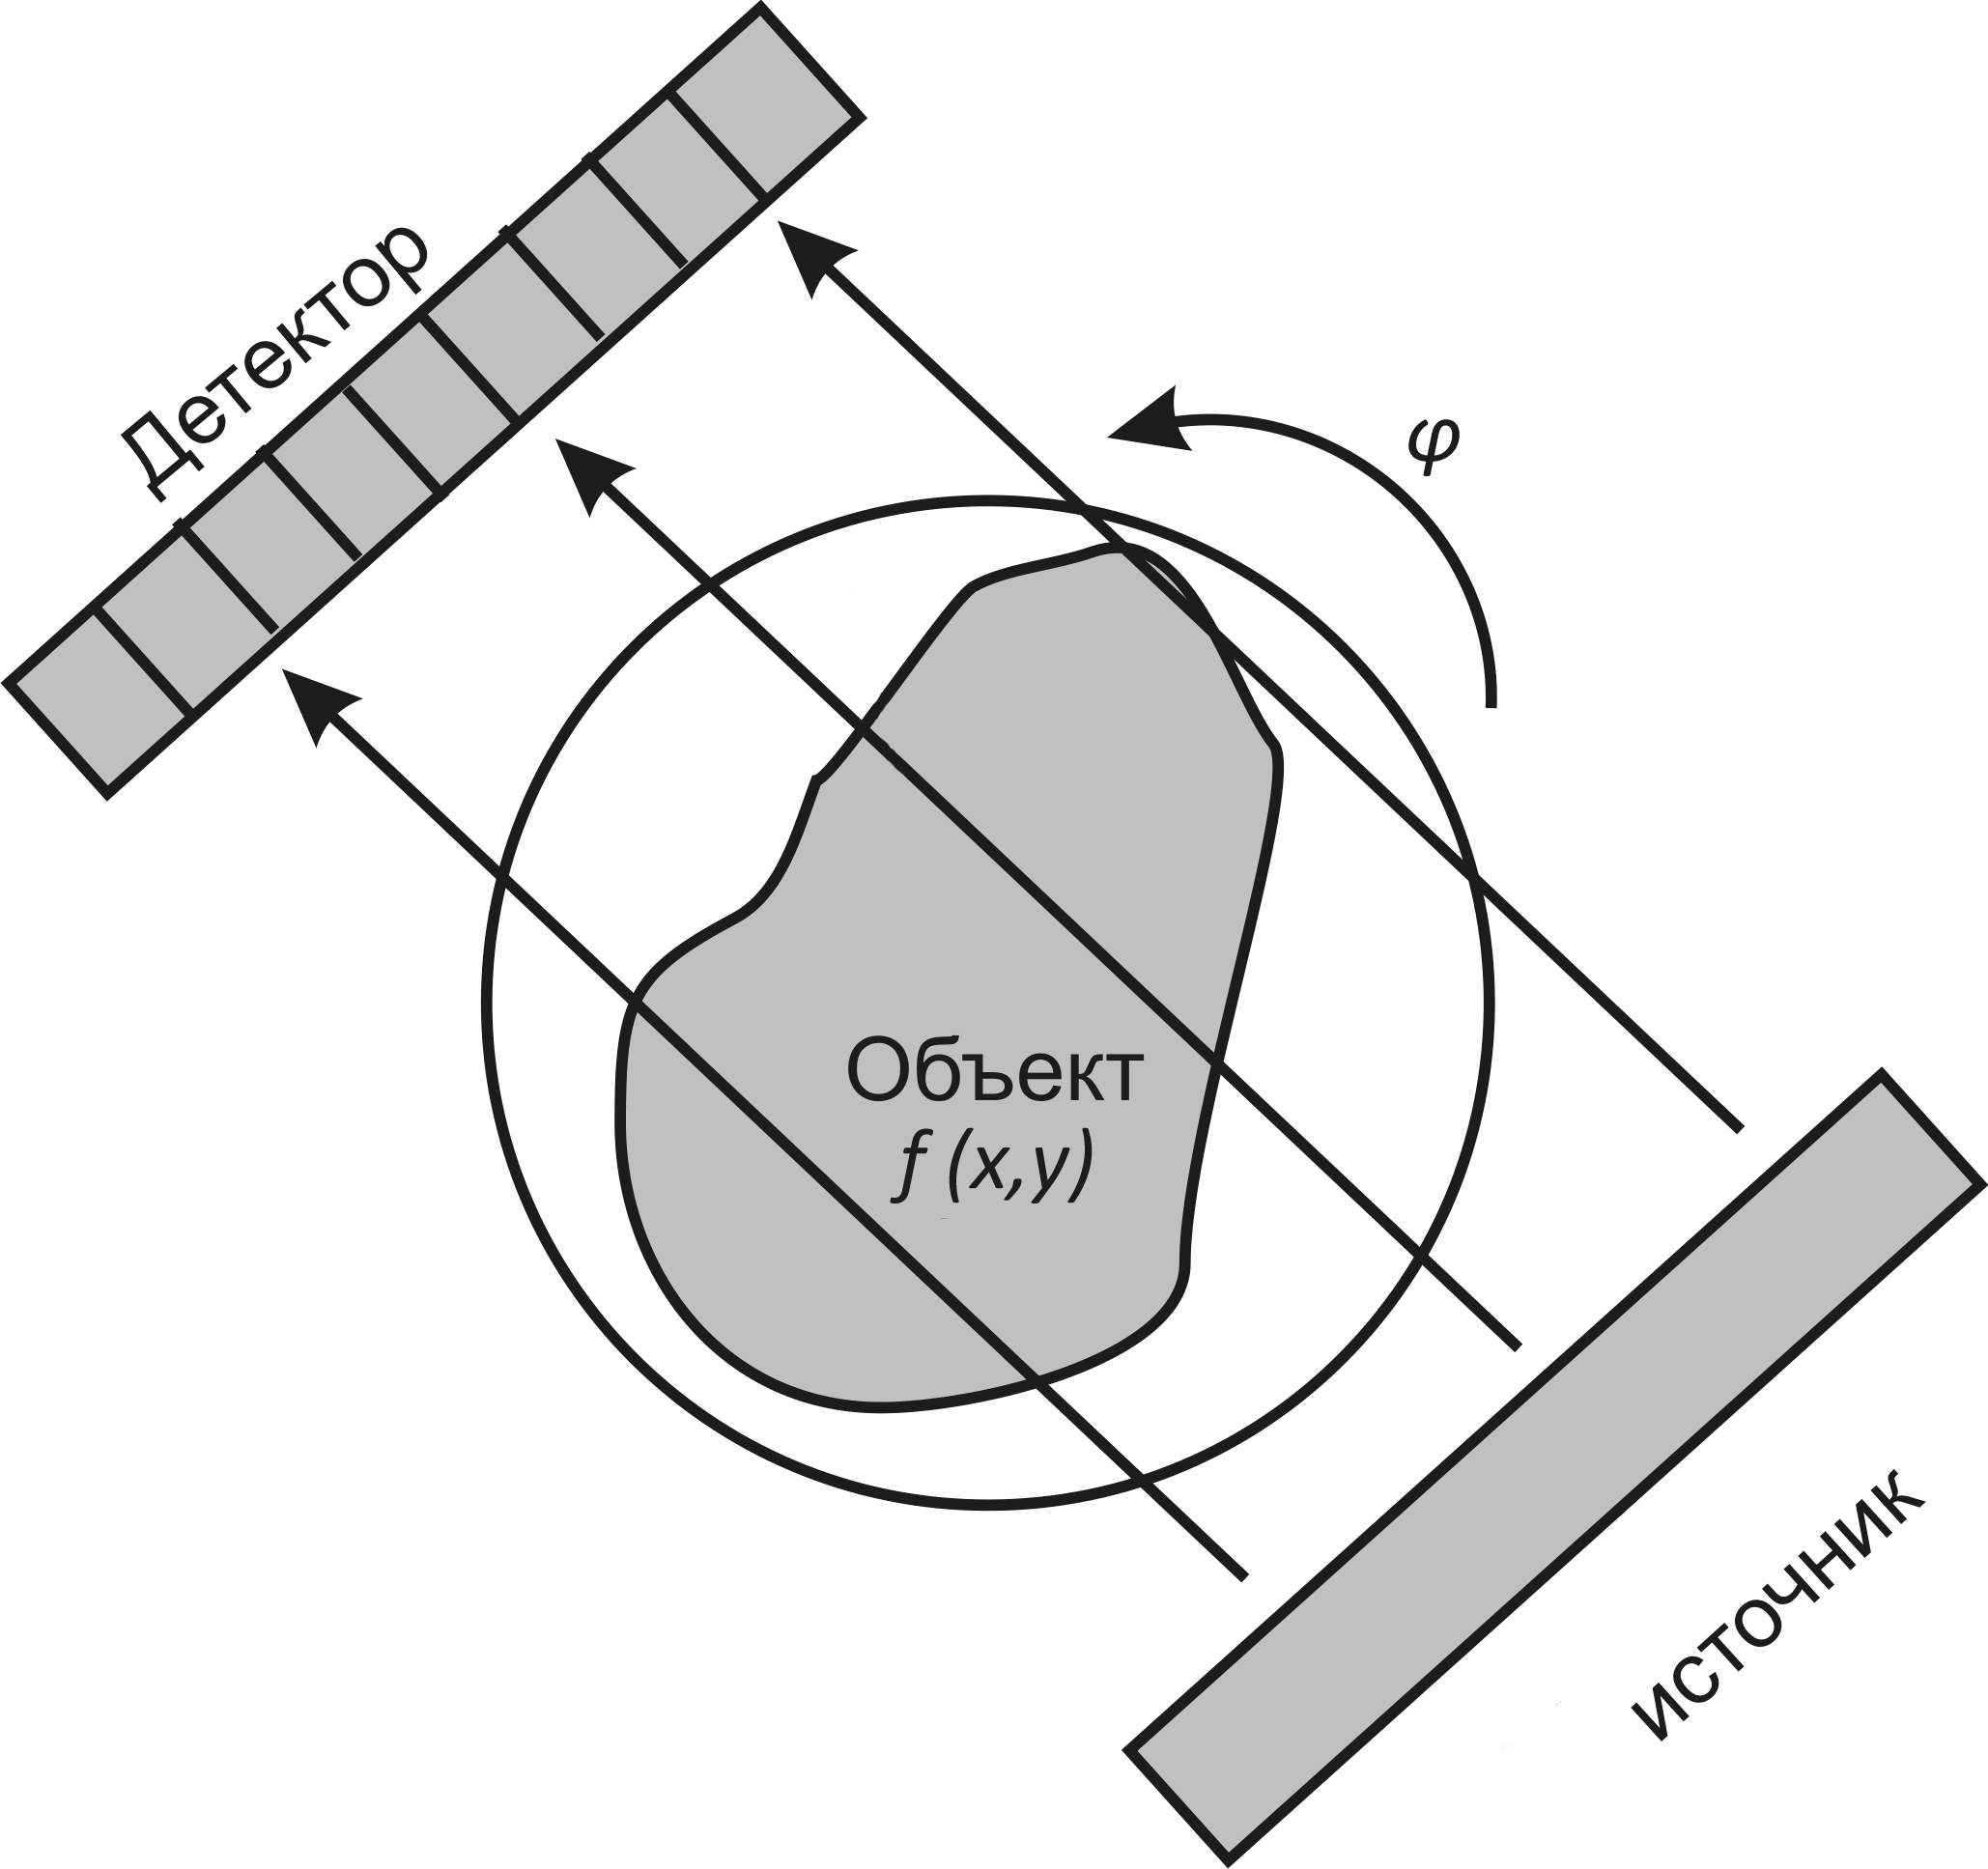
\includegraphics[width=0.45\textwidth]{../Dissertation/images/part1_img/experiment}
  \end{figure}
  &
  \begin{itemize}
  \item $N$ ячеек детектора
  \item $N_\varphi$ углов сканирования
  \item Для каждого угла $\varphi$ и каждой ячейки $\xi$ измеряется интенсивонсть прошедшего рентгеновского излучения \\
    $\mathrm I \left( \varphi, \xi \right) = \mathbb P (f(x, y))$ \\
    $\mathbb P$ --- оператор проекции \\
    $x, y$ --- координаты объекта

  \end{itemize}
\end{tabular}
\end{frame}

\begingroup
% \small

\begin{frame}
% \frametitle{Предмет исследования}
Компьютерная томография --- программно-аппаратный комплекс
% \pause
\setlength{\leftmargini}{0em}
\begin{columns}[T,onlytextwidth]
  \begin{column}{.4\textwidth}
  \begin{itemize}
    \item экспериментальная схема
    \item калибровка 
    \item \textbf{программная обработка $\rightarrow$}
  \end{itemize}
  \end{column}
  \pause
  \begin{column}[t]{0.4\linewidth}
  \begin{itemize}
    \item предобработка
    \item \textbf{алгоритмы восстановления $\rightarrow$}
    \item постобработка
  \end{itemize}
  \end{column}
  \pause
  \begin{column}[t]{0.35\linewidth}
  \begin{itemize}
    \item \textbf{метод оптимизации}
    \item \textbf{модель регуляризации}
    \item \textbf{физическая модель}
    \item реализация математических примитивов
  \end{itemize}
  \end{column}
\end{columns}
\end{frame}
\endgroup

% \begin{frame}
% \frametitle{План доклада}
% \begin{itemize}
% \item Подходы к решению задачи восстановления в КТ
% \item Алгоритм восстановления FHT-SIRT
% \item Учет наличия в объекте высокопоглощающих включений
% \item Метод восвзвешанных невязок
% \end{itemize}
% \end{frame}


\begin{frame}
\frametitle{Предположения}
\begin{itemize}
  \item Рассматривается плоское сечение
  \item Параллельная схема проекции
  \item Ослабление интенсивности излучения подчиняется закону Бугера:
\end{itemize}
  $$
  \mathrm I \left( \varphi, \xi , \lambda \right) = \mathrm I_0(\lambda) \exp\left( {-\int_{l(\varphi, \xi)} \! f(l, \lambda) \mathrm d l }\right),
  $$
  \small
  $f(x, y)$ ---  описывает распределение линейного коэффициента ослабления рентгеновского излучения \\
  $\mathrm I(\varphi, \xi, \lambda)$ --- зарегистрированная детектором интенсивность излучения длины волны $\lambda$ \\
  $\mathrm I_0(\lambda)$ --- интенсивность зондирующего излучения \\
  $l(\varphi, \xi)$ --- параметризация прямой под углом $\varphi$, и сдвигом $\xi$ \\
\end{frame}

\begin{frame}
\frametitle{Задача восстановления}
  Связь линейного коэффициента ослабления и интенсивности описывается преобразованием Радона $R[f(x,y)](\varphi, \xi)$:

  $$
  R[f](\varphi, \xi) = 
 \iint \! \mathrm d x \mathrm d y f(x,y)\delta(x\cos\varphi + y\sin\varphi - \xi)
  $$


  После логарифмирования закона ослабления:
  $$
  \ln \left (\frac{\mathrm I_0(\lambda)}{\mathrm I(\varphi, \xi, \lambda)} \right) = p(\varphi, \xi) = R[f](\varphi, \xi)
  $$

\end{frame}

\begin{frame}
\frametitle{Задача восстановления}
\begin{figure}
\centering
    прямая задача, модель измерения\\
    $\rightarrow$
    \\
    \begin{tabular}{p{0.1\textwidth} p{0.8\textwidth} p{01\textwidth}}
    \hspace{-1cm}
    \small{объект}
    &
    \hspace{-1cm} -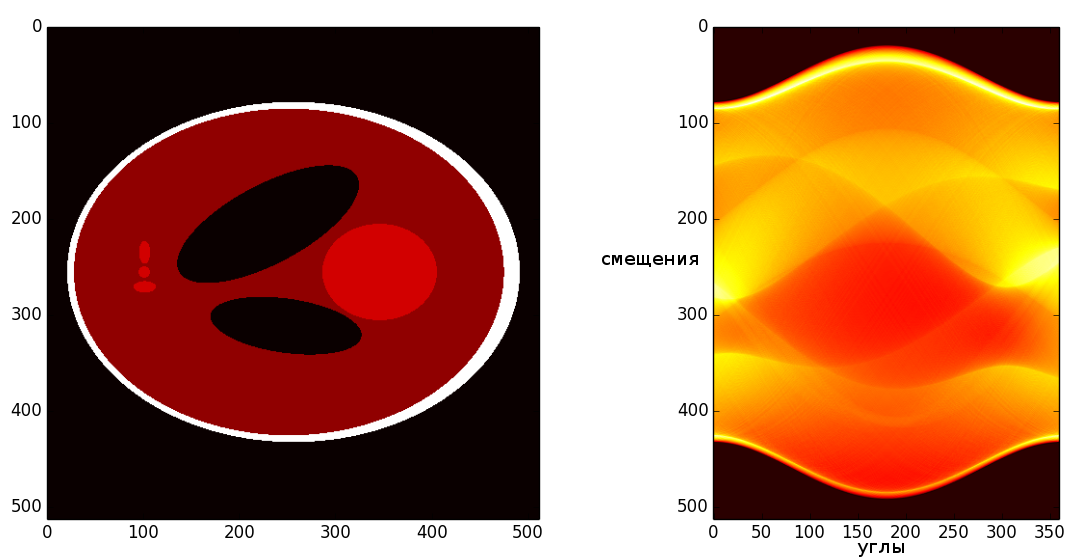
\includegraphics[width=0.8\textwidth]{sl_sinogram}
    &
    \hspace{-1cm} \small{измерения}
    \\
     \hspace{-1cm} \small{$f(x, y)$}
     &
    &
     \hspace{-1cm} \small{$p(\xi, \varphi)$}
    \end{tabular}
    \\
    $\leftarrow$ \\
    обратная задача, процедура восстановления
\end{figure}
\end{frame}

% \begin{frame}
% \frametitle{Задача восстановления}
% 
% Задача восстановления функции $f(x,y)$- задача обращения преобразования Радона полученных измерений $p$:
% $$
% f(x,y) = R^{-1}(p(\varphi, \xi))
% $$
% \end{frame}
